\documentclass[ignorenonframetext,xcolor=x11names]{beamer}

\input{../common.preamble.beamer.tex}
 
\title{Business 4720 - Class 5}

\subtitle{Data Management in R using Tidyverse}

\begin{document}

\begin{frame}{}
  \titlepage
  \footnotesize
  \input{../license.tex}
\end{frame}

\section{Introduction}

\begin{frame}{This Class}

\begin{block}{What You Will Learn:}
\begin{itemize}
  \item Introduction to R
  \item Introduction to the Tidyverse set of packages
  \begin{itemize}
  \item ''Tidy'' data
  \item Manipulating \& cleaning data
  \item Joining data
  \item Summarizing and reporting data
  \end{itemize}
  \item Data cleaning
\end{itemize}
\end{block}
\end{frame}

\section{R}

\begin{frame}{Intro to R}
\begin{block}{What is R?}
\begin{itemize}
  \item System for statistical analyses
  \item Created in 1993
  \item R programming language
  \item Open-source, cross-platform
  \item Widely used, popular
  \item Extensible, thousands of packages
  \item Scripting and programming
\end{itemize}  
\end{block}
\vspace{5mm}
\textbf{Intro Tutorial:}
\url{https://cran.r-project.org/doc/manuals/r-release/R-intro.pdf}
\end{frame}

\begin{frame}{R}
\centering
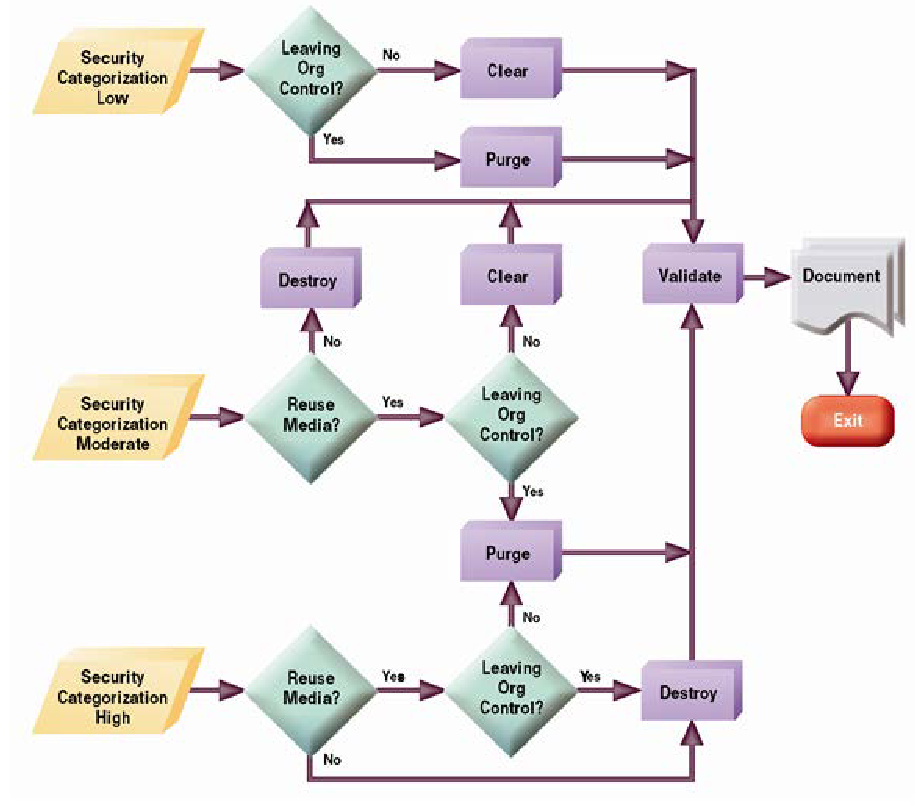
\includegraphics[width=\textwidth]{screen1.png}
\end{frame}

\begin{frame}{Tips for Working with R}

To make using R more efficient, consider doing the following:

\begin{itemize}
    \item Use the {\footnotesize\colorbox{lightgray}{up-arrow}} key to retrieve earlier commands.
    \item The \texttt{history()} function shows your command history.
    \item Use a notepad app to assemble and edit your commands easily, then copy/paste to R for execution.
    \item Use a notepad app for your results, copy/paste from R.
    \item The Ubuntu terminal uses {\footnotesize\colorbox{lightgray}{SHIFT-CTRL-X}}, {\footnotesize\colorbox{lightgray}{SHIFT-CTRL-C}}, {\footnotesize\colorbox{lightgray}{SHIFT-CTRL-V}} for cut/copy/paste.
    \item Use multiple terminal and R windows (e.g. one for executing commands, one for reading help documentation or for listing files).
    \item Don't update packages in the middle of a project.
    \item Ensure you have a \emph{repeatable, automatable script} for your entire data analysis at the end of a project.
\end{itemize}
\end{frame}


\begin{frame}[fragile]{My First R Commands}
R can do math:
\begin{Rcode}
> 1+1
[1] 2
\end{Rcode}
R knows variables:
\begin{Rcode}
> a <- 3
> b <- 2
> print(a * b)
[1] 6
\end{Rcode}
\emph{Note}: You can also assign using ''=''
\end{frame}

\begin{frame}[fragile]{R Basics}
R knows if its not a number:
\begin{Rcode}
> 2 / 0
[1] Inf
> 0 / 0
[1] NaN
\end{Rcode}
\end{frame}

\begin{frame}[fragile]{R Basics \small [cont'd]}
R knows boolean logic:
\begin{Rcode}
> TRUE & FALSE
FALSE
> TRUE | FALSE
TRUE
\end{Rcode}

\emph{Tip}: TRUE and FALSE can be abbreviated T and F \\

R know character strings:
\begin{Rcode}
label1 = 'I Love R'
label2 = 'and BUSI 4760'
paste(label1, label2, sep=' ')
strsplit('Hello World! My first string', ' ')
\end{Rcode}
\emph{Note}: Strings may be enclosed in double or single quotes. \\

\end{frame}

\begin{frame}[fragile]{R Basics \small [cont'd]}
R types and type coercion:
\begin{Rcode}
# Check whether it is numeric
is.numeric(2)
# Check whether it is an integer number
is.integer(3.14)
# Make it an integer
as.integer(3.14)
# Make it a character string
as.character(3.14)
# Make it a character string
as.character(TRUE)
# Make it a number
as.numeric('3.1415')
\end{Rcode}
\end{frame}

\section{The R Environment}

\begin{frame}[fragile]{R Environment}
R can manipulate its objects (''workspace'')
\begin{Rcode}
# Show objects in workspace
> ls()
[1] "a"          "b"          "v"
# Remove one object
> rm(v)
> ls()
[1] "a"          "b"
\end{Rcode}
\end{frame}


\begin{frame}[fragile]{R Environment \small [cont'd]}
R can help:
\begin{Rcode}
help()
help(lm)
?lm
??lm
help.start()
\end{Rcode}
\end{frame}

\begin{frame}[fragile]{R Environment \small [cont'd]}
R has a working directory in which it stores and reads its data:
\begin{Rcode}
# Get the working directory
getwd()
# Set the working directory
setwd('DataSets')
getwd()
# List files in working directory
list.files()
\end{Rcode}

\emph{Tip:} It is often more convenient to change the working directory in the terminal, prior to invoking.

\end{frame}

\begin{frame}[fragile]{R Environment \small [cont'd]}
R uses packages:
\begin{Rcode}
# Install the tidyverse library
install.packages('tidyverse')
# Load/attach the tidyverse library
library(tidyverse)
# List all installed packages
installed.packages()
\end{Rcode}
R can read command files:
\begin{Rcode}
source('MyFirstScript.R')
\end{Rcode}
\emph{Note}: Sourcing a script turns off auto-printing, you must use explicit \texttt{print()} commands
\end{frame}

\begin{frame}[fragile]{R Environment \small [cont'd]}
Say goodbye to R:
\begin{Rcode}
quit()
\end{Rcode}
R stores its \textbf{workspace} in each directory in a file called ''.RData'' and will read it when restarted. R stores its \textbf{command history} in each directory in a file called ''.Rhsitory'' and will read it when restarted.
\end{frame}

\section{Vectors}

\begin{frame}[fragile]{R Vectors}
All elements have the same type:
\begin{Rcode}
> v <- c(1, 'a', TRUE)
> v
[1] "1"    "a"    "TRUE"
\end{Rcode}
R does vector math:
\begin{Rcode}
> v <- c(1, 2, 3, 4)
> v
[1] 1 2 3 4
> v*3
[1]  3  6  9 12
\end{Rcode}
\emph{Note}: No print statement needed in interactive mode

\begin{Rcode}
# Generate a sequence
s <- seq(0, 6, by=.5)
print(s)
# Repeat a value
r <- rep(3.5, 5)
print(r)
\end{Rcode}
\end{frame}

\begin{frame}[fragile]{R Vectors \small [cont'd]}
More basic functions on vectors:
\begin{Rcode}
length(v)
max(v)
min(v)
sqrt(v)
var(v)
sd(v)
# Vectors get flattened
vv <- c(v, c(7, 8, 9), v)
print(vv)
\end{Rcode}
\end{frame}

\begin{frame}[fragile]{R Vectors \small [cont'd]}
Vector indexing:
\begin{Rcode}
vv < 5
vv[vv < 5]
vv[vv < 5] <- vv[vv < 5] + 5
# Indexing is inclusive
vv[3:7]
# Exclude some elements
vv[-(3:7)]
\end{Rcode}

\emph{Important}: R indexes start at 1!

\end{frame}

\begin{frame}[fragile]{R Missing Values}
R knows NA:
\begin{Rcode}
# Introduce a missing value
v[3] <- NA
# Missing value arithmetic
v*3
# Testing for missing values
is.na(v)
# Missing values in aggregate functions
sum(v)
sum(v, na.rm=TRUE)
\end{Rcode}
\end{frame}

\begin{frame}[fragile]{R Vectors \small [cont'd]}
Regular Expressions:
\footnotesize
\begin{Rcode}
# Match/find North American phone numbers
> grep('^([0-9]{3})[ -]?[0-9]{3}[ -]?[0-9]{4}$', 
    c('709 864 5000', 'abc def 9999', '709-865-5000'))
[1] 1 3
# Match/find Canadian postal codes
> grep('[A-V][0-9][A-V] [0-9][A-V][0-9]', 
    c('A0P 1L0', '0AB L2K', 'A0X 1Z0'))
[1] 1
\end{Rcode}
\normalsize
Levenshtein distances:
\footnotesize
\begin{Rcode}
# Match/find strings up to Levenshtein distance of 3
> agrep('apple', 
    c('apricot', 'banana', 'grape', 'pineapple'), 
    max.distance=3)
[1] 1 3 4
\end{Rcode}
\end{frame}

\section{Arrays, Matrices, Lists, and DataFrames}

\begin{frame}[fragile]{R Arrays and Matrices}
Arrays and matrices have dimensions:
\begin{Rcode}
# Default is to fill by column
a <- array(1:20, dim=c(4,5))
a
# Result:
#      [,1] [,2] [,3] [,4] [,5]
# [1,]    1    5    9   13   17
# [2,]    2    6   10   14   18
# [3,]    3    7   11   15   19
# [4,]    4    8   12   16   20
# Indexing is inclusive and starts at 1
a[,2]
a[,2:4]
a[3,2:4]
a[3:1,2:4]
\end{Rcode}
\end{frame}

\begin{frame}{R Arrays and Matrices \small [cont'd]}
\begin{itemize}
   \item The first dimension is the row, the second is the column
   \item Initially, the array is created from a range of numbers between 1 and 20, and the \texttt{dim} argument specifies the dimensionality. 
   \item R fills arrays by column, unless otherwise specified
   \item A dimension need not be slided or indexed, as in \texttt{a[,2]} or \texttt{a[,2:4]} which do not subset the first dimension (rows). The result is that all rows are returned in these examples. 
   \item Reversing the index reverses the result that is returned, as in \texttt{a[3:1,2:4]} which reverses the indexing of the first dimension (rows). 
\end{itemize}
\end{frame}

\begin{frame}[fragile]{R Arrays and Matrices \small [cont'd]}
\begin{Rcode}
b <- matrix(20:1, nrow=5, byrow=T)
b
# Result:
#      [,1] [,2] [,3] [,4]
# [1,]   20   19   18   17
# [2,]   16   15   14   13
# [3,]   12   11   10    9
# [4,]    8    7    6    5
# [5,]    4    3    2    1
# Test if it is a matrix
is.matrix(b)
is.matrix(a)
# Transpose
t(b)
# Bind (combine) by columns
cbind(a, t(b))
# Bind (combine) by rows
rbind(t(a), b)
\end{Rcode}
\end{frame}

%\begin{frame}[fragile]{R Lists}
%R knows lists:
%\begin{Rcode}
%l <- list('a', 3, 'b', 2, TRUE)
%l[[2]]
%l[2]
%is.list(l)
%is.list(l[[2]])
%is.list(l[2])
%as.list(vv)
%\end{Rcode}
%\emph{Vectors are not lists}: Lists can contain elements of different types, vectors cannot:
%\begin{Rcode}
%c(3, 'a', TRUE)
%c(3, FALSE, TRUE)
%\end{Rcode}
%\end{frame}


\begin{frame}[fragile]{R Data Frames}
\begin{Rcode}
# Create a vector of 50 normally distributed random variables
x <- rnorm(50)
# Create another vector with random variables
y <- 2*x + rnorm(50)
# Create a data frame from the two vectors
data <- data.frame(x, y)
#  Get the column names
colnames(data)
# Update the column names
colnames(data) <- c('Pred', 'Crit')
# Get the number of rows and columns
nrow(data)
ncol(data)
# Get the "Pred" column of the data frame
data$Pred
# Print a summary
summary(data)
# Print first and last rows
head(data)
tail(data)
# Calculate the covariance matrix
cov(data)
\end{Rcode}
\end{frame}


\begin{frame}[fragile]{Data Frames \small [cont'd]}
Writing data to CSV:
\begin{Rcode}
# Write CSV file into current working directory
# Omit the row names
write.csv(data, 'data.csv', row.names=FALSE)
\end{Rcode}

Reading data from CSV:
\begin{Rcode}
# Read the data from the current working directory
new.data <- read.csv('data.csv')
\end{Rcode}
\end{frame}

\begin{frame}{Hands-On Exercise}
\begin{enumerate}
   \item Create an array with $3$ columns and $50$ rows of random numbers with mean of $2$ and standard deviation of $4$ (use the \texttt{rnorm()} function)
   \item Create a dataframe from the array and name the columns as ''A'', ''B'', ''C''
   \item ''Clip'' the values so that all values lie between $-3$ and $+7$
   \item Summarize the data 
   \item Print the pairwise covariance matrix of the three columns in the data frame
   \item Find the square root of each of the diagonal entries of the covariance matrix, compare this to the standard deviation of 4. Tip: Use the \texttt{diag()} function.
   \item Save the data frame in a CSV file using your first name as file name (file ending '.csv')
\end{enumerate}
\end{frame}

\section{Tidyverse}

\begin{frame}{Tidyverse}
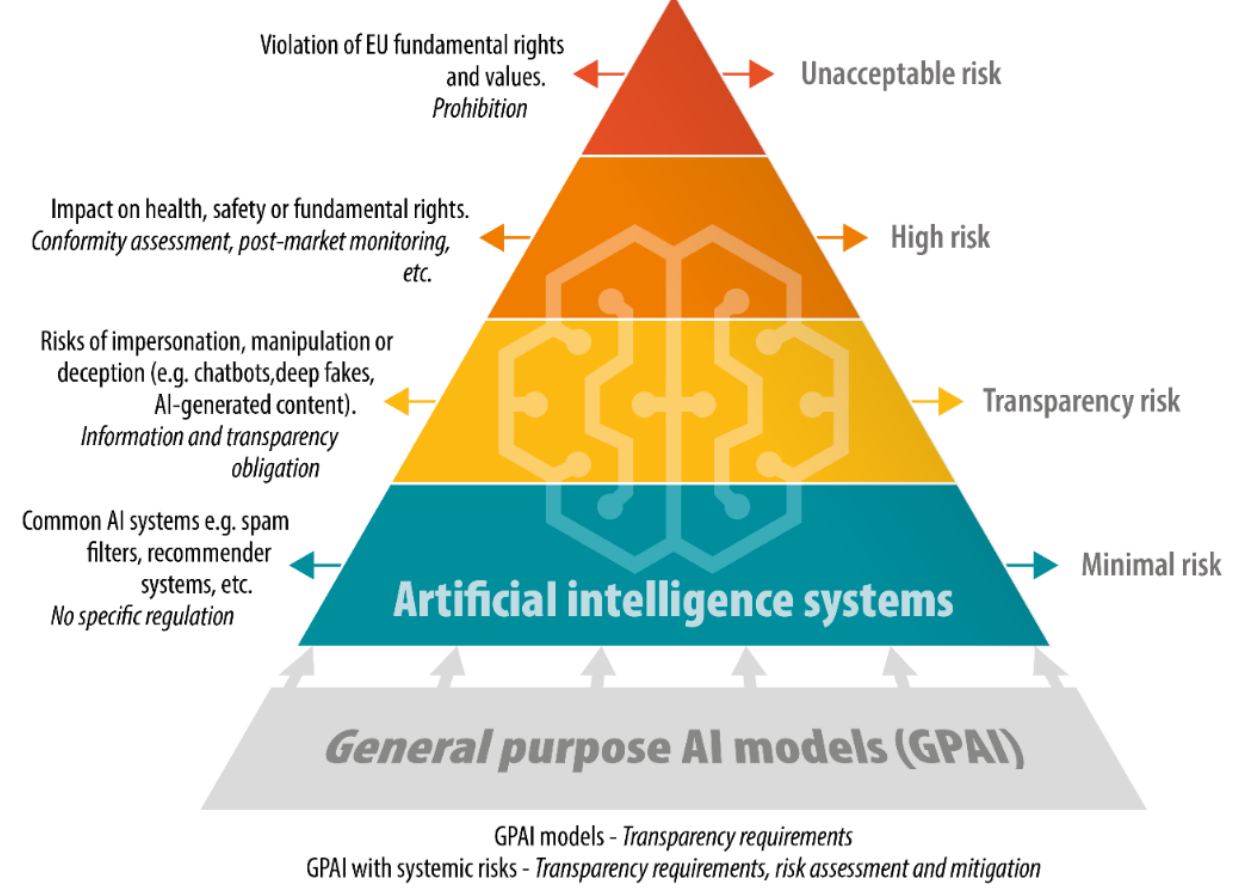
\includegraphics[width=\textwidth]{screen2.png}\\

\textbf{Intro books}: \url{https://r4ds.hadley.nz/} \\

\textbf{''Cheat sheets}: \url{https://posit.co/resources/cheatsheets/} 
\end{frame}

\begin{frame}{Tidyverse Packages}
\renewcommand{\arraystretch}{1.25}
\centering

\begin{tabular}{l|l} \hline
dplyr & Manipulate data \\
forcats & Work with categorical variables (factors) \\
ggplot2 & Grammar of Graphics \\
lubridate & Date and time parsing and arithmetic \\
purrr & Functional programming \\
readr & Read files in various formats \\
stringr & Work with character strings \\
tibble & A tibble is better than a table \\
tidyr & Make data tidy \\ \hline
\end{tabular}
\end{frame}

\begin{frame}{Example Dataset}
\begin{itemize}
  \item Government of Canada, Open Government Portal
  \item Fuel Consumption Ratings -- Battery-electric vehicles -- 2012--2023
  \item \href{https://open.canada.ca/data/en/dataset/98f1a129-f628-4ce4-b24d-6f16bf24dd64}{https://open.canada.ca/data/en/dataset/98f1a129-f628-4ce4-b24d-6f16bf24dd64}
\end{itemize} 

\vspace{\baselineskip}
\centering
\footnotesize

	\begin{tabular}{|l|l|} \hline
	  {\bf Column} & {\bf Data Type} \\ \hline \hline
	  Make & Categorical (string) \\ 
	  Model & Categorical (string) \\
	  Year & Numeric \\
	  Category & Categorical (string)\\
	  City & Numeric \\
	  Hwy & Numeric \\
	  Comb & Numeric \\
	  Range & Numeric \\ \hline
	\end{tabular}
\end{frame}

\begin{frame}[fragile]{Read Data}
Load Tidyverse library and read data into a ''tibble''

\begin{Rcode}
# Load library
library(tidyverse)
# Read CSV into a Tibble
data <- read_csv('https://evermann.ca/busi4720/fuel.csv')
# Examine the data
# Dimensions (rows, columns)
dim(data)
# Column names
colnames(data)
# Summary
summary(data)
\end{Rcode}

Tibbles are an extension of data frames and provide more capabilities. Tibbles and data frames are automatically converted into each other when required.
\end{frame}


\begin{frame}{Summary of DPlyr ''Verbs''}

\footnotesize
\centering
\renewcommand{\arraystretch}{1.25}

\begin{tabularx}{\textwidth}{l|X} \hline
\multicolumn{2}{c}{Basic} \\ \hline
\texttt{filter} & filters by row \\
\texttt{select} & selects columns to retain \\
\texttt{mutate} & creates new columns \\
\texttt{rename} & renames columns \\
\texttt{distinct} & finds unique values \\
\texttt{arrange} & sorts data rows \\
\texttt{relocate} & moves data columns \\
\texttt{group\_by} & groups data \\
\texttt{summarize} & compute aggregate information \\
\texttt{print} & prints a tibble \\  \hline
\multicolumn{2}{c}{Advanced} \\ \hline
\texttt{nest} & nests data, tibbles in tibbles \\
\texttt{full\_join} & Joins tibbles (also \texttt{outer join}, \texttt{left\_join}, \texttt{inner\_join}, \texttt{right\_join}) \\ \hline
\end{tabularx}

\end{frame}

\begin{frame}[fragile]{Filter()}

Filters data based on conditions:

\begin{Rcode}
# Pipe a data frame or tibble into a filter and print results
data |> 
  filter(Make=='Ford', Year==2023) |> 
  print()

# Equivalent without pipe and boolean operator in filter
filter(data, Make=='Ford' & Year==2023)
\end{Rcode}

Equivalent SQL:

\begin{sqlcode}
SELECT * 
   FROM data 
   WHERE Make=='Ford' AND Year==2023;
\end{sqlcode}

\end{frame}

\begin{frame}[fragile]{Select()}

Selects specified columns:

\begin{Rcode}
# Pipe a data frame or tibble into a filter,
# select specific columns and print results
data |> 
  filter(Make=='Ford', Year==2023) |> 
  select(Model, Category, Range) |>
  print()
\end{Rcode}

Equivalent SQL:

\begin{sqlcode}
SELECT Model, Category, Range 
   FROM data 
   WHERE Make=='Ford' AND Year==2023;
\end{sqlcode}
\end{frame}

\begin{frame}[fragile]{Mutate()}

Creates new calculated columns:

\begin{Rcode}
# Pipe a data frame or tibble into a filter,
# create a new calculated column,
# select specific columns and print results
data |> 
  filter(Make=='Ford', Year==2023) |> 
  mutate(HwyRange = Range * Comb / Hwy) |>
  select(Model, Category, Range, HwyRange) |>
  print()
\end{Rcode}

Equivalent SQL:

\begin{sqlcode}
SELECT Model, Category, Range, (Range*Comb)/Hwy AS HwyRange 
   FROM data 
   WHERE Make=='Ford' AND Year==2023;
\end{sqlcode}
\end{frame}

\begin{frame}[fragile]{Rename()}

Renames columns:

\begin{Rcode}
# Pipe a data frame or tibble into a filter,
# create new calculated columns,
# rename an existing column,
# select specific columns and print results
data |> 
  filter(Make=='Ford', Year==2023) |> 
  mutate(HwyRange = Range * Comb / Hwy) |>
  mutate(CityRange = Range * Comb / City) |>
  rename(CombRange = Range) |>
  select(Model, Category, CombRange, CityRange, HwyRange) |>
  print()
\end{Rcode}

Equivalent SQL:

\begin{sqlcode}
SELECT Model, Category, 
      Range AS CombRange,
      (Range*Comb)/Hwy AS HwyRange, 
      (Range*Comb)/City As CityRange
   FROM data 
   WHERE Make=='Ford' AND Year==2023;
\end{sqlcode}
\end{frame}

\begin{frame}[fragile]{Distinct()}

Returns unique values:

\begin{Rcode}
# Pipe a data frame or tibble into a filter,
# select distinct value combinations and print results
data |> 
  distinct(Make, Model) |>
  print()
\end{Rcode}

Equivalent SQL:

\begin{sqlcode}
SELECT DISTINCT Make, Model 
  FROM data;
\end{sqlcode}
\end{frame}

\begin{frame}[fragile]{Arrange()}

Sorts/orders data by value:

\begin{Rcode}
# Pipe a data frame or tibble into a filter,
# select specific columns,
# order the data and print results
data |> 
  filter(Make=='Ford', Year==2023) |> 
  select(Model, Category, Range) |>
  arrange(Category, desc(Range)) |>
  print()
\end{Rcode}

Equivalent SQL:

\begin{sqlcode}
SELECT Model, Category, Range
   FROM data 
   WHERE Make=='Ford' AND Year==2023
   ORDER BY Category ASC, Range DESC;
\end{sqlcode}
\end{frame}

\begin{frame}[fragile]{Relocate()}

Reorders columns:

\begin{Rcode}
# Pipe a data frame or tibble into a filter,
# select specific columns,
# order the data,
# move columns and print results
data |> 
  filter(Make=='Ford', Year==2023) |> 
  select(Model, Category, Range) |>
  arrange(Category, desc(Range)) |>
  relocate(Category, Range) |>
  print()
\end{Rcode}

Equivalent SQL:

\begin{sqlcode}
SELECT Category, Range, Model
   FROM data 
   WHERE Make=='Ford' AND Year==2023
   ORDER BY Category ASC, Range DESC;
\end{sqlcode}
\end{frame}

\begin{frame}[fragile]{Group\_by() and summarize()}

Groups data and calculates summary values for each group:

\begin{Rcode}
# Pipe a data frame or tibble into a filter,
# group the data
# summarize the data,
# filter the summary information,
# order the data,
# relocate columns and print results
data |> 
  filter(Year==2023) |> 
  group_by(Make, Category) |>
  summarize(meanCity = mean(City), 
            meanHwy = mean(Hwy),
            meanComb = mean(Comb),
            maxRange = max(Range),
            nVehicle = n()) |>
  filter(nVehicle > 1) |>
  arrange(Category, meanComb) |>
  relocate(Category, meanComb) |>
  print()
\end{Rcode}
\end{frame}

\begin{frame}[fragile]{Group\_by() and summarize()}

Equivalent SQL:

\begin{sqlcode}
SELECT Category, 
       AVG(Comb) AS meanComb,
       Make,
       AVG(City) AS meanCity,
       AVG(Hwy) AS meanHwy,
       MAX(Range) AS maxRange,
       COUNT(*) AS nVehicle
   FROM data 
   WHERE Year==2023
   GROUP BY Make, Category
   HAVING COUNT(*) > 1
   ORDER BY Category ASC, meanComb ASC;
\end{sqlcode}
\end{frame}



\begin{frame}[fragile]{Pagila Database in R}
Read data into tibbles:
\small
\begin{Rcode}
rentals <- read_csv('http://evermann.ca/busi4720/rentals.csv')
actors <- 
  read_csv('https://evermann.ca/busi4720/actors.categories.csv')
addresses <- 
  read_csv('https://evermann.ca/busi4720/addresses.csv')
\end{Rcode}

Fix the column datatypes:

\footnotesize
\begin{Rcode}
attach(rentals)
rating <- as.factor(rating)
language <- as.factor(language)
customer_address <- as.integer(customer_address)
customer_store <- as.integer(customer_store)
rental_staff <- as.integer(rental_staff)
payment_staff <- as.integer(payment_staff)
rental_duration <- as.integer(rental_duration)
detach(rentals)

addresses$phone <- as.character(addresses$phone)
\end{Rcode}
\end{frame}

\begin{frame}[fragile]{Pagila Database in R \small [cont'd]}
Examine the NA's:
\footnotesize
\begin{Rcode}
rentals |> 
  filter(if_any(everything(), is.na)) |>
  select(last_name, rental_date, return_date, 
         title, amount) |>
  print(n=Inf, width=Inf)
\end{Rcode}
\normalsize
\emph{Interpretation:}
\begin{itemize}
  \item Some films have not been rented
  \item Some rentals have not been returned
\end{itemize}
\end{frame}

\begin{frame}[fragile]{Pagila Database in R \small [cont'd]}

Find all films and the actors that appeared in them, ordered by film category and year, for those films that are rated PG:

\scriptsize
\begin{Rcode}
rentals |> 
    full_join(actors, 
        by='title', 
        suffix=c('_customer', '_actor'), 
        relationship='many-to-many') |>
    filter(rating == 'PG') |>
    mutate(actor = 
        paste(last_name_actor, ', ', 
        first_name_actor, sep='')) |>
    rename(year=release_year) |>
    select(actor, title, category, year) |>
    distinct(actor, title, category, year) |>
    group_by(category, year, title) |> 
    nest() |>
    arrange(category, year, title) |>
    relocate(category, year, title) |>
    print(n=Inf, width=Inf)
\end{Rcode}
\end{frame}

\begin{frame}[fragile]{Pagila Database in R \small [cont'd]}

Find the most popular actors in the rentals in each city:

\scriptsize
\begin{Rcode}
rentals |> 
   inner_join(addresses,
       by=c('customer_address'='address_id')) |>
   inner_join(actors,
       by='title',
       suffix=c('_customer', '_actor'),
       relationship='many-to-many') |>
   mutate(actor = 
       paste(last_name_actor, ', ', 
       first_name_actor, sep='')) |>
   group_by(city, actor) |>
   summarize(count=n()) |>
   mutate(ranking = min_rank(desc(count))) |>
   filter(ranking < 4) |>
   arrange(city, ranking, actor) |>
   print(n=25)
\end{Rcode}

\normalsize
\emph{Note}: Use \texttt{rank()} to break ties, \texttt{dense\_rank()} for no gaps
\end{frame}

\begin{frame}[fragile]{Pagila Database in R \small [cont'd]}

Find the customers who spend the most on rentals, with their phone numbers and cities, and the number of rentals with the higest total rental payments for each category grouped by rental duration.

\footnotesize
\begin{Rcode}
full_data <- 
   rentals |> 
     inner_join(addresses,
       by=c('customer_address'='address_id')) |>
     inner_join(actors,
       by='title',
       suffix=c('_customer', '_actor'),
       relationship='many-to-many')
\end{Rcode}
\end{frame}

\begin{frame}[fragile]{Pagila Database in R \small [cont'd]}
\footnotesize
\begin{Rcode}
full_data |>
   mutate(customer=
     paste(first_name_customer, last_name_customer)) |>
   select(customer, amount, rental_duration, 
          category, phone, city) |>
   group_by(category, rental_duration, customer ) |>
   mutate(payments=sum(amount), num_rentals=n()) |>
   select(-amount) |>
   group_by(category, rental_duration) |>
   mutate(ranking = min_rank(desc(payments))) |>
   slice(which.min(ranking)) |>
   print(n=Inf, width=Inf)
\end{Rcode}
\normalsize

\begin{itemize}
  \item No \texttt{summarize()}
  \item ''Negative'' \texttt{select()}
  \item Multiple \texttt{group\_by()}
  \item Uses \texttt{slice()}
\end{itemize}
\end{frame}

\begin{frame}[fragile]{Pagila Database in R \small [cont'd]}
Get the total rental revenue, number of rentals, and the mean and standard deviation of the rental amounts for each country.

\footnotesize
\begin{Rcode}
full_data |>
  group_by(country) |>
  summarize(revenue=sum(amount), 
            numrentals=n(),
            mean_amount=mean(amount),
            sd_amount=sd(amount)) |>
  arrange(desc(mean_amount),
          desc(revenue)) |>
  print(n=Inf, width=Inf)  
\end{Rcode}
\normalsize
\end{frame}

\begin{frame}[fragile]{Pagila Database in R \small [cont'd]}
Get the top 5 and the bottom 5 grossing customers for each quarter.

\footnotesize
\begin{Rcode}
full_data |>
  mutate(customer=
   paste(first_name_customer,last_name_customer)) |>
  mutate(q=
   as.character(quarter(rental_date, with_year=T))) |>
  select(customer, q, amount, rental_date) |>
  group_by(q, customer) |>
  mutate(payments=sum(amount)) |>
  select(-amount) |>
  distinct(customer, q, payments) |>
  group_by(q) |>
  mutate(rank_top = min_rank(desc(payments))) |>
  mutate(rank_bot = min_rank(payments)) |>
  filter(rank_top < 6 | rank_bot < 6) |>
\end{Rcode}
\end{frame}

\begin{frame}[fragile]{Pagila Database in R \small [cont'd]}
Continued from previous slide \ldots

\footnotesize
\begin{Rcode}
  arrange(q, desc(payments)) |>
  relocate(q, customer, payments, 
              rank_top, rank_bot) |>
  print(n=Inf, width=Inf)
\end{Rcode}
\normalsize
\begin{itemize}
  \item No \texttt{summarize()}
  \item Uses \texttt{quarter()} function from package \texttt{lubridate}
  \item Uses \texttt{filter()} instead of slice \texttt{slice()}
\end{itemize}
\end{frame}


\begin{frame}[fragile]{Pagila Database in R \small [cont'd]}

Find the set of film titles by rental customer and the total number rentals for each customer

\footnotesize
\begin{Rcode}
full_data |>
  mutate(customer=
    paste(first_name_customer,last_name_customer)) |>
  select(customer, title) |>
  nest(titles=title) |>
  rowwise() |> 
  mutate(rentals=nrow(titles)) |>
  mutate(unique_titles=list(distinct(titles))) |>
  select(-titles) |>
  arrange(customer)
\end{Rcode}
\normalsize

\begin{itemize}
  \item Work with nested data using \texttt{nest} and \texttt{rowwise}
\end{itemize}
\end{frame}


\begin{frame}{Hands-On Exercises}
\begin{enumerate}
  \item Find all films with a rating of 'PG'
  \item List all customers who live in Canada (with their address)
  \item Find the average \emph{actual} rental duration for all films
  \begin{itemize}
     \item This requires date arithmetic, use the \texttt{lubridate} package
  \end{itemize}
  \item Find the average overdue time for each customer
  \begin{itemize}
     \item This requires date arithmetic, use the \texttt{lubridate} package
  \end{itemize}
  \item List all films that have never been rented
  \item List the names of actors who have played in more than 15 films
\end{enumerate}
\end{frame}

\begin{frame}[fragile]{R knows SQL}

\begin{block}{The \texttt{sqldf} Package}
  \begin{itemize}
     \item Set up an in-memory SQLite database (or use existing database connection)
     \item Move dataframes to database tables
     \item Run SQL query against database
     \item Move result set to R dataframe
     \item Tear down the in-memory database (optional)
  \end{itemize}
\end{block}

\begin{block}{Example}
\small
\begin{Rcode}
library(sqldf)
result_df <- 
   sqldf('select distinct(title) from full_data')
\end{Rcode}
\end{block}
\end{frame}


\begin{frame}{SQL Databases versus R/Tidyverse}
\begin{block}{Consider:}
  \begin{itemize}
     \item \textbf{Size of data}: R is memory limited, RDBMS scale massively larger
     \item \textbf{Access speed}: RDBMS have sophisticated indexes and query planners
     \item \textbf{Currency}: Operational system RDBMS has live data
     \item \textbf{Transactions}: RDBMS ensure consistent views of data across multi-user, concurrent updates
     \item \textbf{Impact}: Queries impact transaction processing (updates of data) performance in RDBMS 
     \item \textbf{Tools}: R has tools for statistical analysis and visualization, beyond mere reporting
  \end{itemize}
\end{block}
\end{frame}

\begin{frame}{SQL Databases versus R/Tidyverse \small [cont'd]}
\begin{block}{Recommendations:}
  \begin{itemize}
     \item Do not ''hit'' operational RDBMS for heavy-weight or frequent analytics
     \item Regularly export consistent data from RDBMS
     \item Use separate in-memory or on-disk RDBMS for analytics (e.g. with \texttt{sqldf}) if desired/required
     \item If size of data is large, consider distributed tools such as Hadoop/Spark
  \end{itemize}
\end{block}
\end{frame}

\end{document}
